\newpage
%================================================================
\section{Results and Discussion}\label{sec:Results}
%================================================================

% simple figure
\begin{figure}[!htb]
\begin{center}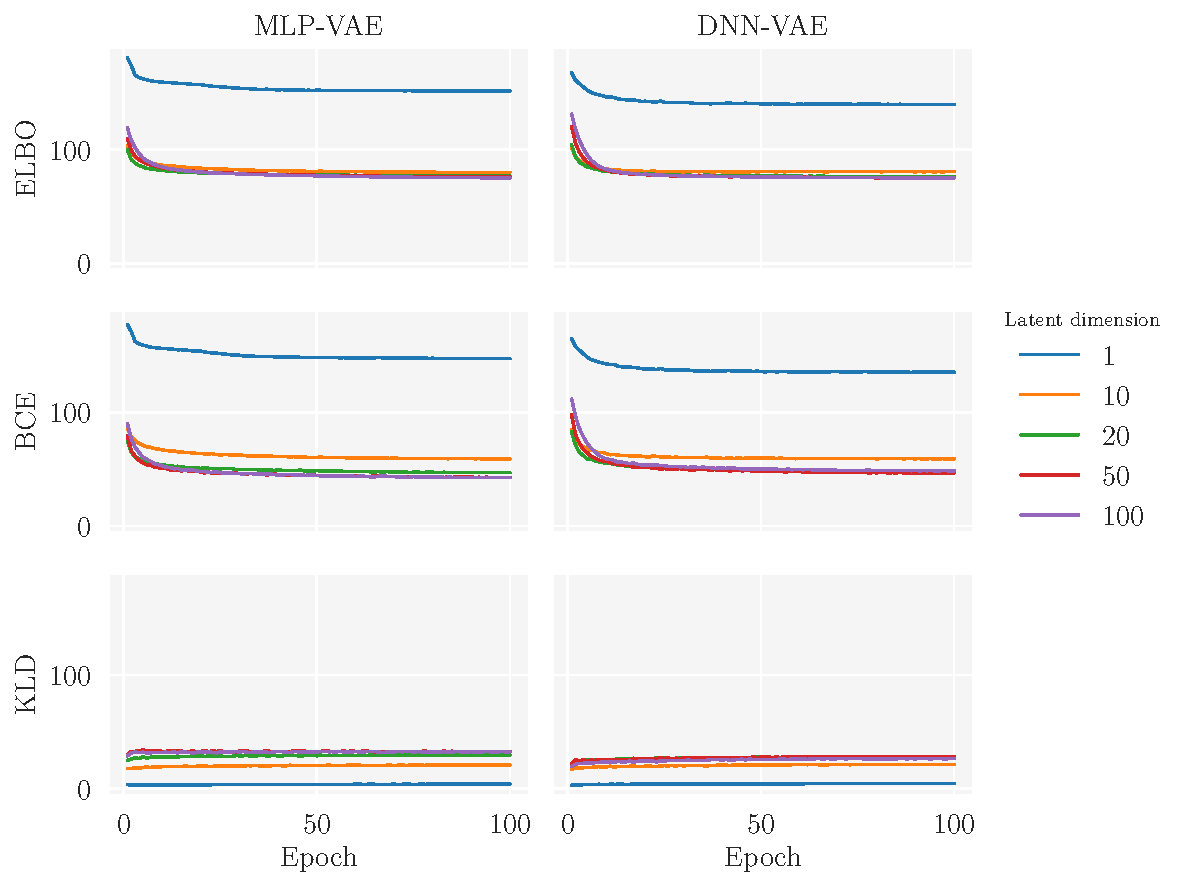
\includegraphics[scale=0.7]{latex/figures/loss_latent_dim_vanilla_mlp_dnn_vae_bmnist.pdf}
\end{center}
\caption{figure text}
\label{fig:loss_latent_dim_vanilla_mlp_dnn_vae_bmnist}
\end{figure}


\begin{figure}[!htb]
\centering
\subfloat[]{{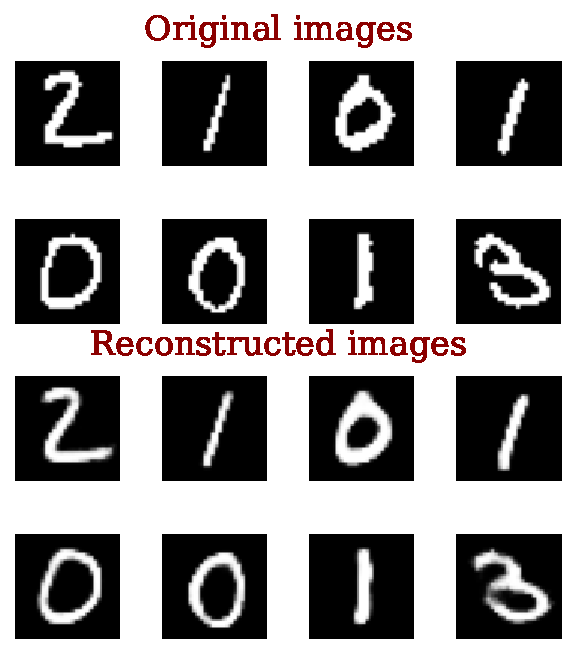
\includegraphics[scale=0.5]{latex/figures/recon_latent_dim_20_vanilla_mlp_vae_bmnist.pdf}}}
\qquad
\subfloat[]{{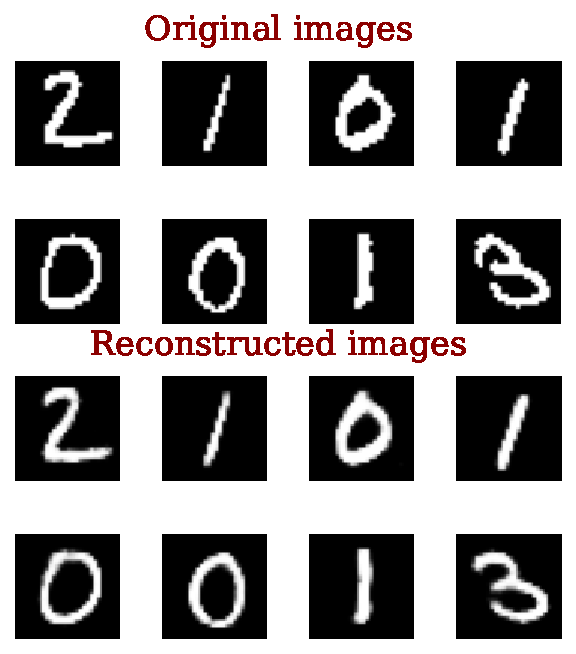
\includegraphics[scale=0.5]{latex/figures/recon_latent_dim_20_vanilla_dnn_vae_bmnist.pdf}}}
\qquad
\subfloat[]{{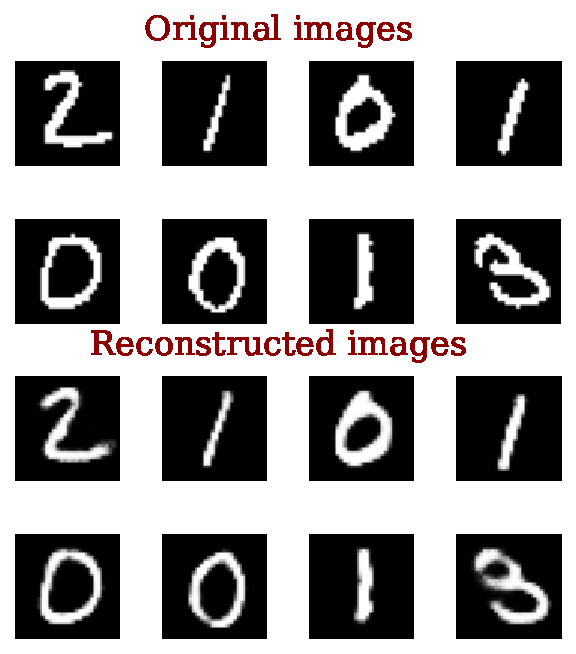
\includegraphics[scale=0.5]{latex/figures/recon_latent_dim_100_vanilla_mlp_vae_bmnist.pdf}}}
\qquad
\subfloat[]{{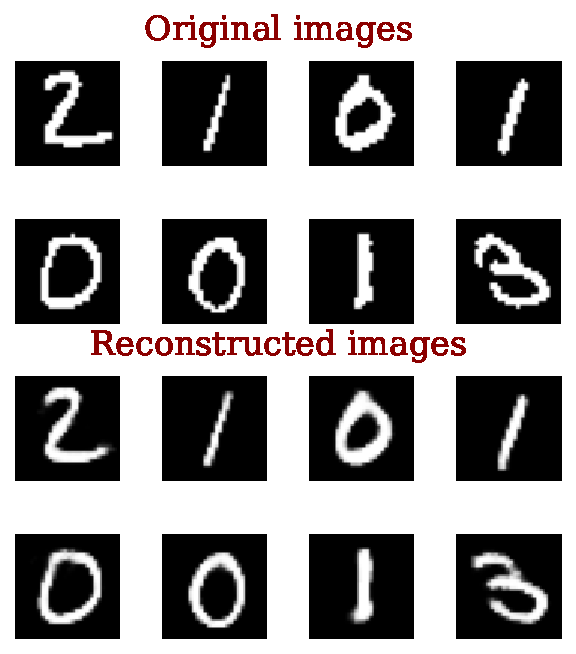
\includegraphics[scale=0.5]{latex/figures/recon_latent_dim_100_vanilla_dnn_vae_bmnist.pdf}}}
\caption{figure text}
\label{fig:recon_latent_dim_vanilla_mlp_dnn_vae_bmnist}
\end{figure}

suggests that VAEs based on a MLP or DNN architecture is not optimal for learning latent representations of the MNIST digits.

%----------------------------------------------------------------
\subsection{Results 1}\label{sec:project results}
%----------------------------------------------------------------

%\FloatBarrier


\url{https://uvadlc-notebooks.readthedocs.io/en/latest/tutorial_notebooks/JAX/tutorial9/AE_CIFAR10.html}

% Comparing latent dimensionality

% When training an autoencoder, we need to choose a dimensionality for the latent representation. The higher the latent dimensionality, the better we expect the reconstruction to be. However, the idea of autoencoders is to compress data. Hence, we are also interested in keeping the dimensionality low. To find the best tradeoff, we can train multiple models with different latent dimensionalities. The original input has 32x32x3 = 3072 pixels. Keeping this in mind, a reasonable choice for the latent dimensionality might be between 64 and 384:

% Clearly, the smallest latent dimensionality can only save information about the rough shape and color of the object, but the reconstructed image is extremely blurry and it is hard to recognize the original object in the reconstruction. With 128 features, we can recognize some shapes again although the picture remains blurry. The models with the highest two dimensionalities reconstruct the images quite well. The difference between 256 and 384 is marginal at first sight but can be noticed when comparing, for instance, the backgrounds of the first image (the 384 features model more of the pattern than 256).

% The encoder and decoder networks we chose here are relatively simple. Usually, more complex networks are applied, especially when using a ResNet-based architecture. For example, see VQ-VAE and NVAE